\chapter{Materiales y Métodos}

\section{Materiales}
\label{section4:materials}
Para la realización de este TFM se dispone de una colección de 497 mallas 3D de la sínfisis del pubis, correspondientes tanto al lado izquierdo como derecho, en formato de malla OBJ. Estas mallas fueron escaneados por el personal del Laboratorio de Antropología Física del Departamento de Medicina Legal, Toxicología y Antropología Física de la Universidad de Granada. Además de la digitalización tridimensional, el equipo del laboratorio examinó cuidadosamente cada una de las muestras y etiquetó manualmente los atributos correspondientes a las características morfológicas observables en la superficie de la sínfisis del pubis así como la edad real de fallecimiento de los individuos, datos que también han sido provistos dentro de un fichero de Microsoft Excel. Se utilizaron las características y atributos propuestos por Villar et al. \cite{villar2017first}, que se pueden visualizar en la Tabla \ref{table:themBones}.


\begin{figure}[htbp]
    \centering
    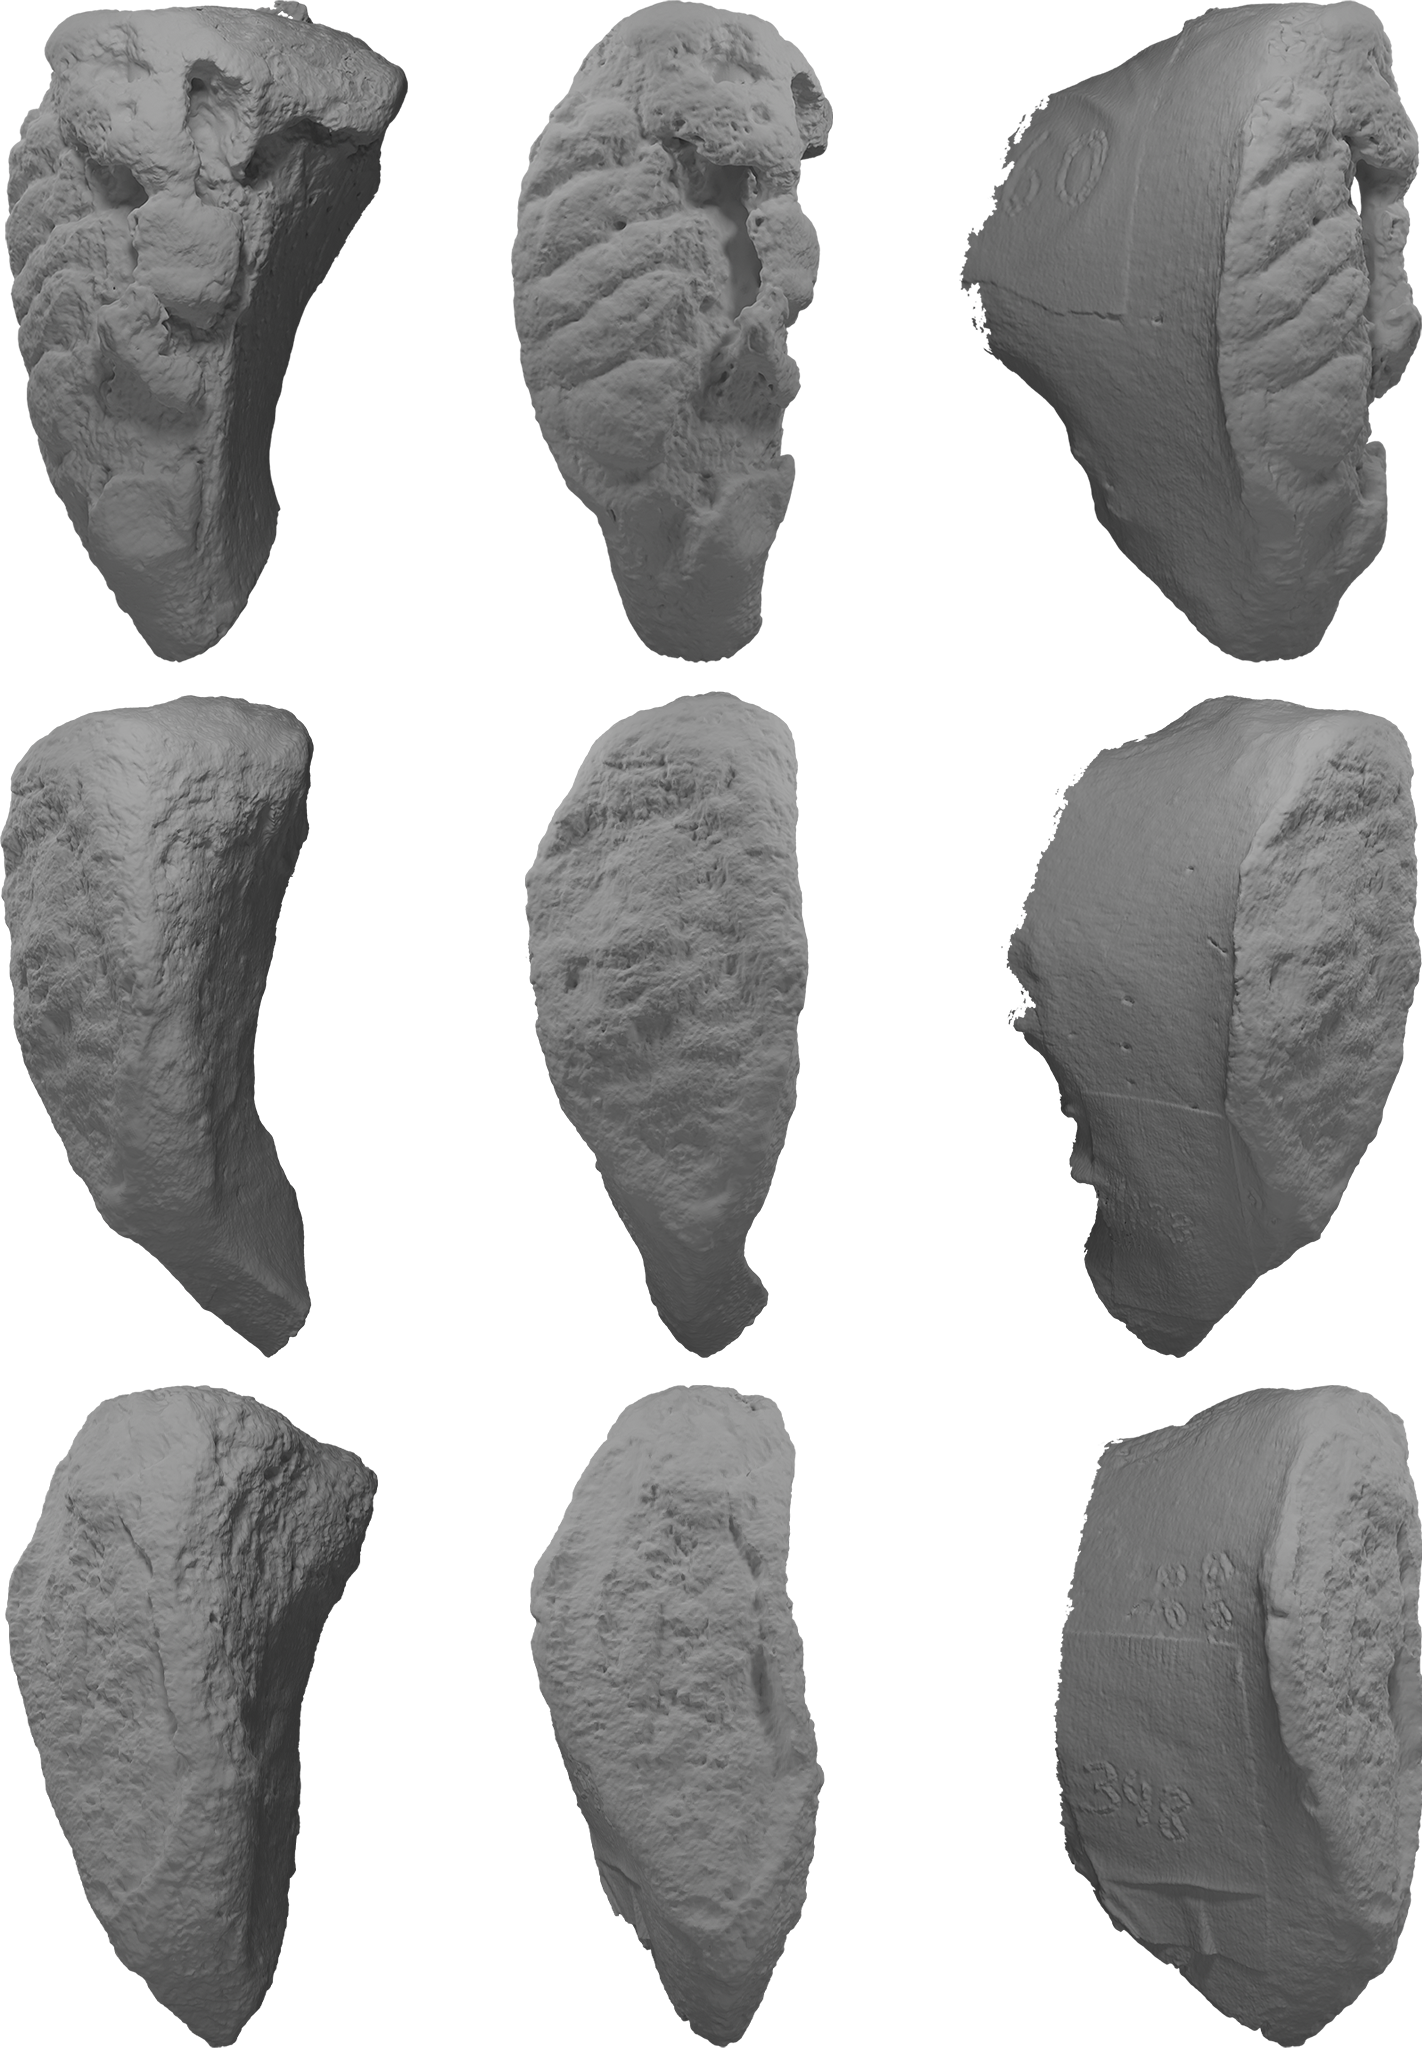
\includegraphics[width=0.75\linewidth]{figures/4_materials-methods/pb-examples.png}
    \caption[Ejemplos de mallas 3D de la sínfisis del pubis]{Ejemplos de mallas 3D de la sínfisis del pubis. Se presentan tres muestras distintas, renderizadas con iluminación fotorrealista desde tres ángulos: vista lateral izquierda (a), frontal (b) y lateral derecha (c). Obsérvese la complejidad de la superficie ósea, la cual ha sido capturada con alta fidelidad por el escáner 3D.}
    \label{pb_3dexamples}
\end{figure}

A partir de este punto, se utilizarán las abreviaciones en inglés de dichas características con el fin de facilitar legibilidad del texto. La correspondencia entre las abreviaciones y su nombre en castellano puede consultarse en la Tabla \ref{table4:chars_short_names}.

\begin{table}[h]
    \centering
    \begin{tabular}{|c|c|c|}
    \hline
    \rowcolor[HTML]{D33333} 
    {\color[HTML]{FFFFFF} Nombre Castellano} & {\color[HTML]{FFFFFF} Nombre Inglés} & {\color[HTML]{FFFFFF} Abreviación} \\ \hline
    Crestas y Surcos & \textit{Auricular Face} & \textbf{AF} \\ \hline
    Porosidad Irregular & \textit{Irregular Porosity} & \textbf{IP} \\ \hline
    Borde Superior & \textit{Upper Symphysial Extremity} & \textbf{USE} \\ \hline
    Nódulo Óseo & \textit{Bony Nodule} & \textbf{BN} \\ \hline
    Borde Inferior & \textit{Lower Symphysial Extremity} & \textbf{LSE} \\ \hline
    Borde Dorsal & \textit{Dorsal Margin} & \textbf{DM} \\ \hline
    Plataforma Dorsal & \textit{Dorsal Plateau} & \textbf{DP} \\ \hline
    Bisel Ventral & \textit{Ventral Bevel} & \textbf{VB} \\ \hline
    Borde Ventral & \textit{Ventral Margin} & \textbf{VM} \\ \hline
    \end{tabular}
    \caption{Correspondencia entre nombres de las características de Todd en castellano e inglés junto con su abreviación.}
    \label{table4:chars_short_names}
\end{table}

\begin{figure}[h]
    \centering
    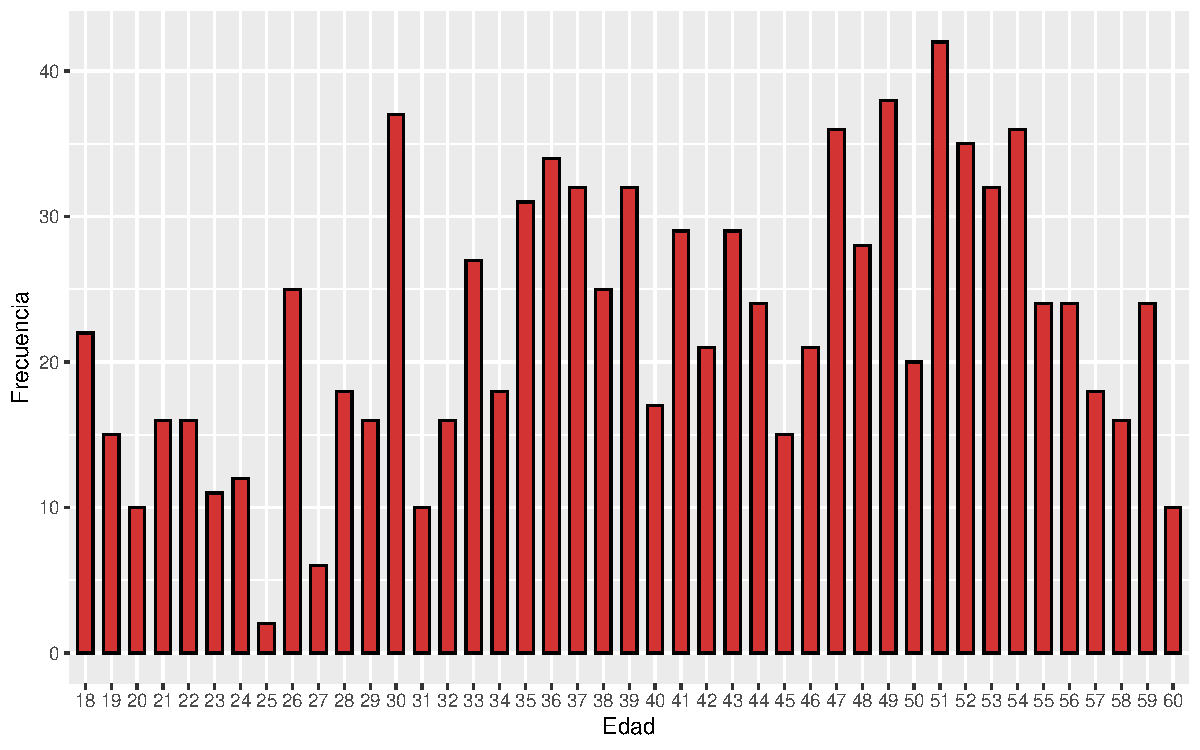
\includegraphics[width=\linewidth]{../../scripts/eda/eda_univar/char_age_distr.pdf}
    \caption[Distribución de los datos por edad]{Distribución de los datos según la edad real de los individuos. Se observa una mayor concentración de muestras en los rangos superiores a los 35 años.}
    \label{fig4:age}
\end{figure}
\begin{figure}[h]
    \centering
    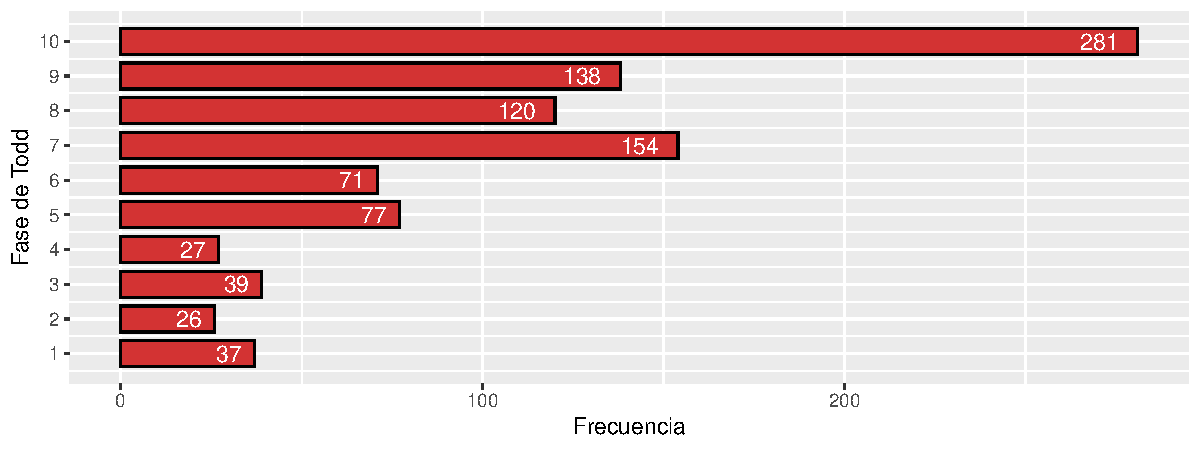
\includegraphics[width=\linewidth]{../../scripts/eda/eda_univar/char_t_phase_distr.pdf}
    \caption[Distribución de los datos por cada rango de edad]{Distribución de los datos por cada rango de edad del método de Todd. Se observa una mayor concentración de muestras entre las fases 7 y 10. Leyenda: \textbf{1}: 18-19 años, \textbf{2}: 20-21 años, \textbf{3}: 22-24 años, \textbf{4}: 25-26 años, \textbf{5}: 27-30 años, \textbf{6}: 30-35 años, \textbf{7}: 35-39 años, \textbf{8}: 39-44 años, \textbf{9}: 45-50 años, \textbf{10}: 50+ años.}
    \label{fig4:todd_phase}
\end{figure}

\subsection{Análisis Exploratorio de Datos}
\label{section4:data_eda}
Realizando un análisis exploratorio de los datos (\textit{Exploratory Data Analysis}, EDA), resulta de interés realizar una inspección visual preliminar de las mallas. En la Figura \ref{pb_3dexamples} se muestran tres mallas 3D de la sínfisis del pubis renderizados con iluminación fotorrealista desde tres ángulos diferentes: vista lateral izquierda, frontal y lateral derecha. A partir de estas imágenes puede observarse que se trata de mallas 3D de alta complejidad geométrica y nivel de detalle. Además, al tratarse de estructuras anatómicas reales, presentan una alta variabilidad morfológica tanto en dimensiones como en proporciones, lo cual supone un reto adicional para los métodos de DL a aplicar.

Cabe destacar que el método seleccionado (ExMeshCNN, véase \ref{section4:methods}) no ha sido validado con datos de esta naturaleza, sino con conjuntos de datos sintéticos y de menor resolución. Aun así, se espera que su rendimiento se mantenga elevado, dado que está diseñado para capturar patrones discriminativos directamente desde la superficie de las mallas, independientemente de su nivel de complejidad o del origen biológico de las estructuras representadas.

Centrándose ahora en los datos asociados a cada malla, se observa que la muestra está compuesta por individuos de entre 18 y 60 años, como se muestra en la Figura \ref{fig4:age}. Además, estos individuos han sido clasificados dentro de las 10 fases del método de Todd, tal como se aprecia en la Figura \ref{fig4:todd_phase}.

De ambos gráficos se aprecia que las edades más representadas corresponden a individuos de mayor edad, lo cual es coherente considerando el origen de los datos. Sin embargo, este patrón también evidencia un desbalance inherente en la muestra, un fenómeno esperado cuando se trabaja con datos reales.

\subsubsection{Análisis Univariable}
Continuando con el EDA enfocado en las nueve características del método de Todd, se observa un claro desbalance en la distribución de atributos, como se muestra en las gráficas correspondientes en la Figura \ref{fig4:todd_chars}. Los atributos más representados son coherentes con las manifestaciones morfológicas que el hueso de la sínfisis del pubis presenta a edades más avanzadas.

Desde la perspectiva del balance de datos, las características USE (Subfigura \ref{fig4:todd_chars__use}), BN (Subfigura \ref{fig4:todd_chars__bn}), DP (Subfigura \ref{fig4:todd_chars__dp}) y LSE (Subfigura \ref{fig4:todd_chars__lse}) presentan un desbalance particularmente acentuado, con aproximadamente 95\%, 91\%, 90\% y 90\% de las muestras concentradas en un solo atributo, respectivamente. Este fuerte desbalance sugiere que estas características podrían tener un rendimiento limitado al ser utilizadas para el entrenamiento de modelos de DL.

\begin{figure}[p]
    \centering
    \begin{subfigure}{\textwidth}
        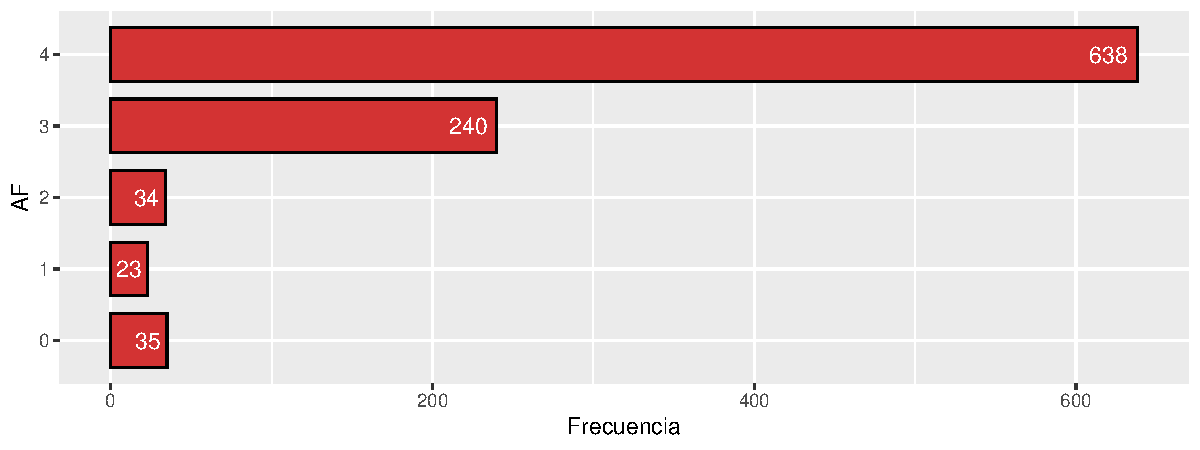
\includegraphics[width=\linewidth]{../../scripts/eda/eda_univar/char_af_distr.pdf}
        \caption{Característica AF. Leyenda: \textbf{0}: Porosidad Regular, \textbf{1}: Muy Definidas, \textbf{2}: Poco Profundas, \textbf{3}: Restos de Surcos, \textbf{4}: No hay surcos.}
        \label{fig4:todd_chars__af}
    \end{subfigure}

    \begin{subfigure}{\textwidth}
        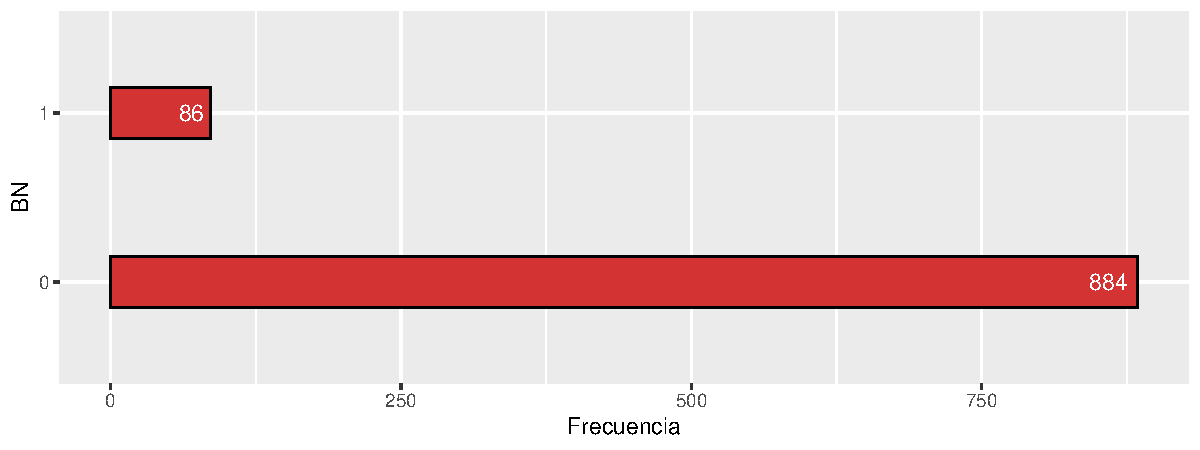
\includegraphics[width=\linewidth]{../../scripts/eda/eda_univar/char_bn_distr.pdf}
        \caption{Característica BN. Leyenda: \textbf{0}: Ausente, \textbf{1}: Presente.}
        \label{fig4:todd_chars__bn}
    \end{subfigure}
    
    \begin{subfigure}{\textwidth}
        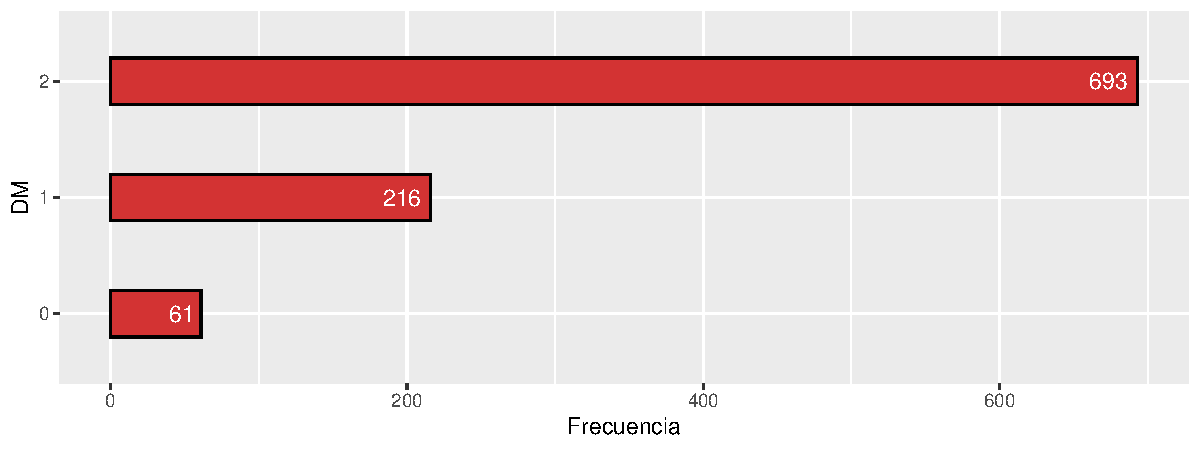
\includegraphics[width=\linewidth]{../../scripts/eda/eda_univar/char_dm_distr.pdf}
        \caption{Característica DM. Leyenda: \textbf{0}: No Definido, \textbf{1}: En Formación, \textbf{2}: Definido.}
        \label{fig4:todd_chars__dm}
    \end{subfigure}
    \phantomcaption

\end{figure}
\begin{figure}[p]
    \ContinuedFloat

    \begin{subfigure}{\textwidth}
        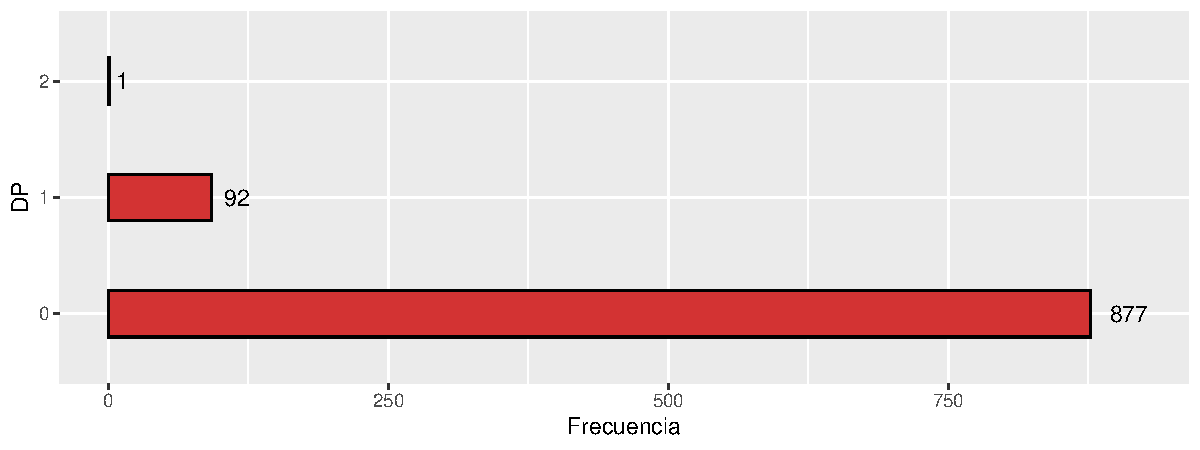
\includegraphics[width=\linewidth]{../../scripts/eda/eda_univar/char_dp_distr.pdf}
        \caption{Característica DP. Leyenda: \textbf{0}: Ausente, \textbf{1}: En Formación, \textbf{2}: Presente.}
        \label{fig4:todd_chars__dp}
    \end{subfigure}

    \begin{subfigure}{\textwidth}
        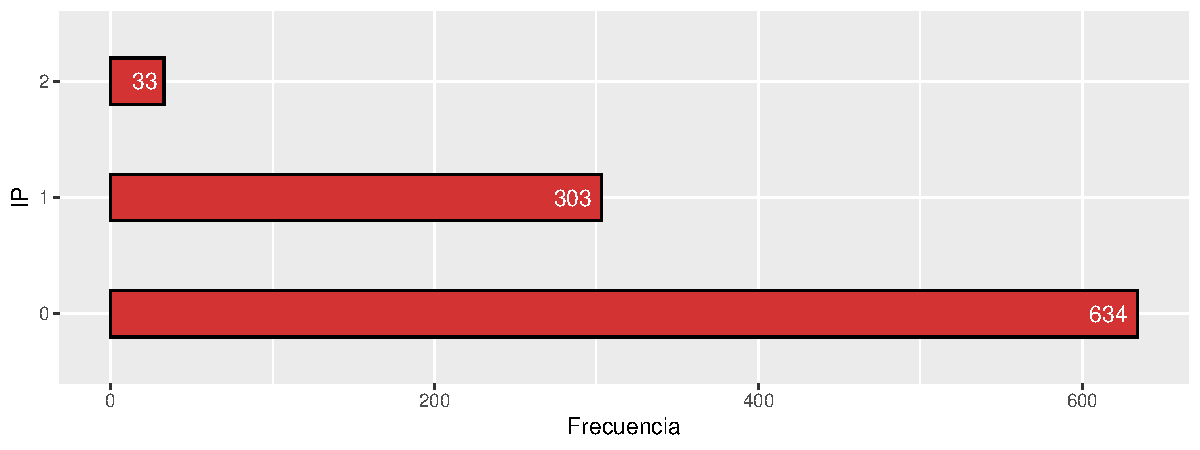
\includegraphics[width=\linewidth]{../../scripts/eda/eda_univar/char_ip_distr.pdf}
        \caption{Característica IP. Leyenda: \textbf{0}: No, \textbf{1}: Mediana, \textbf{2}: Sí.}
        \label{fig4:todd_chars__ip}
    \end{subfigure}

    \begin{subfigure}{\textwidth}
        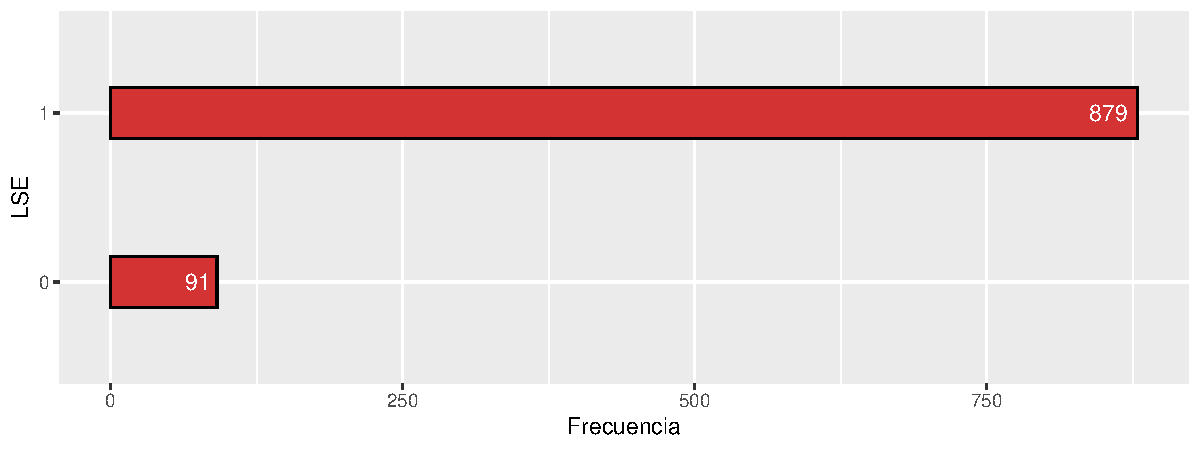
\includegraphics[width=\linewidth]{../../scripts/eda/eda_univar/char_lse_distr.pdf}
        \caption{Característica LSE. Leyenda: \textbf{0}: No Definido, \textbf{1}: Definido.}
        \label{fig4:todd_chars__lse}
    \end{subfigure}

    \phantomcaption
    \label{fig4:todd_chars}
\end{figure}
\begin{figure}[p]
    \ContinuedFloat

    \begin{subfigure}{\textwidth}
        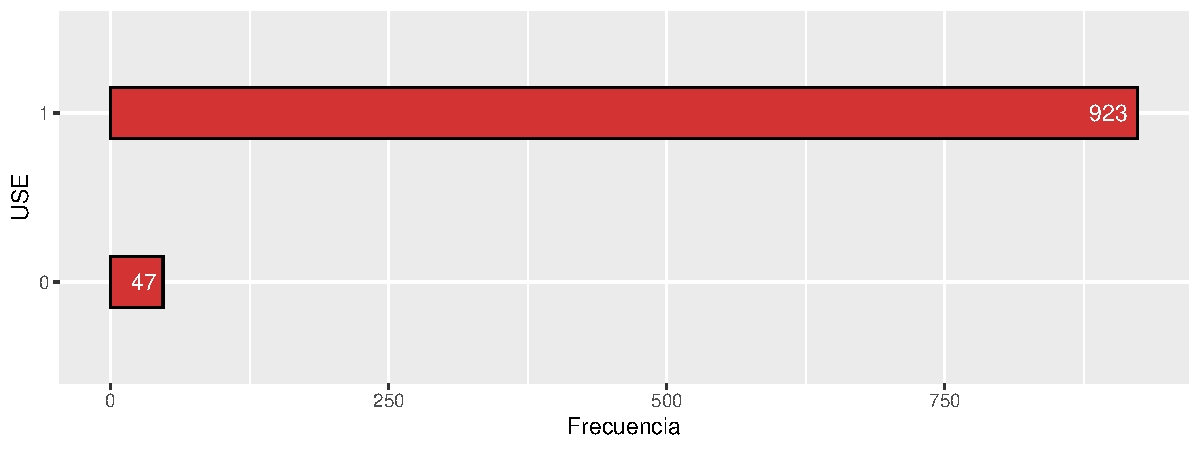
\includegraphics[width=\linewidth]{../../scripts/eda/eda_univar/char_use_distr.pdf}
        \caption{Característica USE. Leyenda: \textbf{0}: No Definido, \textbf{1}: Definido.}
        \label{fig4:todd_chars__use}
    \end{subfigure}

    \begin{subfigure}{\textwidth}
        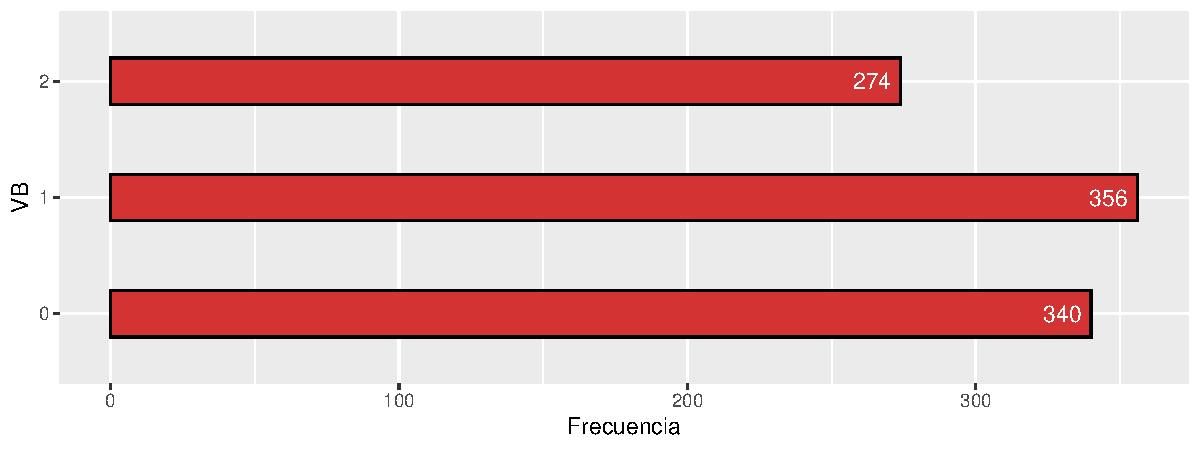
\includegraphics[width=\linewidth]{../../scripts/eda/eda_univar/char_vb_distr.pdf}
        \caption{Característica VB. Leyenda: \textbf{0}: Ausente, \textbf{1}: En Formación, \textbf{2}: Presente.}
        \label{fig4:todd_chars__vb}
    \end{subfigure}

    \begin{subfigure}{\textwidth}
        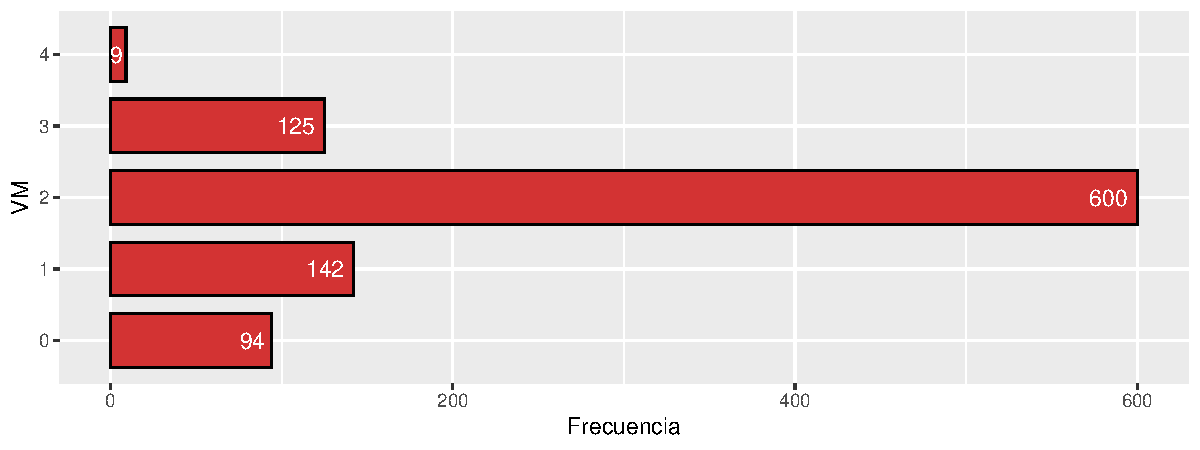
\includegraphics[width=\linewidth]{../../scripts/eda/eda_univar/char_vm_distr.pdf}
        \caption{Característica VM. Leyenda: \textbf{0}: Ausente, \textbf{1}: En Formación, \textbf{2}: Formado, Sin Excrecencias, \textbf{3}: Formado, Pocas Excrecencias, \textbf{4}: Formado, Muchas Excrecencias.}
        \label{fig4:todd_chars__vm}
    \end{subfigure}
    \caption[Distribución de las características de Todd]{Distribución de las etiquetas para cada característica de Todd en el conjunto de datos. Para cada característica, se muestran las frecuencias de las diferentes clases observadas en los datos disponibles. Esta visualización permite apreciar el grado de desbalance entre clases y la variabilidad presente en cada rasgo morfológico.}

\end{figure}

El resto de las características muestra un desbalance menos extremo, con entre el 60\% y el 70\% de los datos agrupados en una único atributo. La característica con mayor equilibrio en su distribución es el VB (Subfigura \ref{fig4:todd_chars__vb}), en la que los datos se reparten aproximadamente en un 33\% por atributo, dado que esta posee tres atributos distintos. Se espera que esta característica, junto con aquellas que presenten menos desbalance, proveerán mejores resultados al ser entrenadas por la red.

\subsubsection{Correlaciones}

\begin{figure}[p]
    \centering
    \begin{subfigure}{\textwidth}
        \centering
        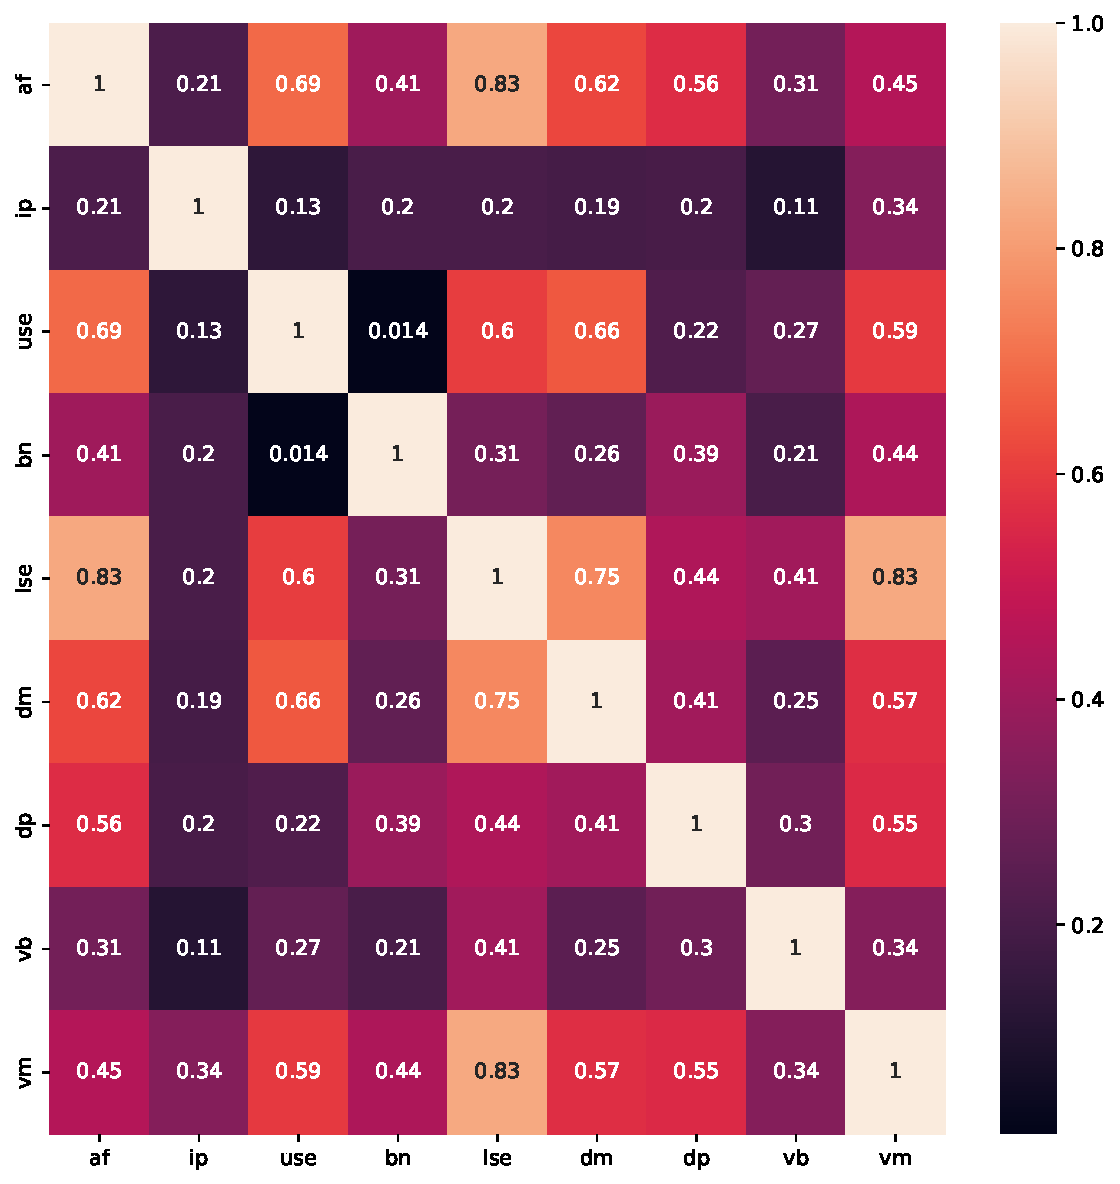
\includegraphics[width=0.6\linewidth]{../../scripts/eda/assoc_plot_cramersv.pdf}
        \caption{Mapa de calor de la V de Cramér}
        \label{fig4:todd_chars__cramersv}
    \end{subfigure}
    \begin{subfigure}{\textwidth}
        \centering
        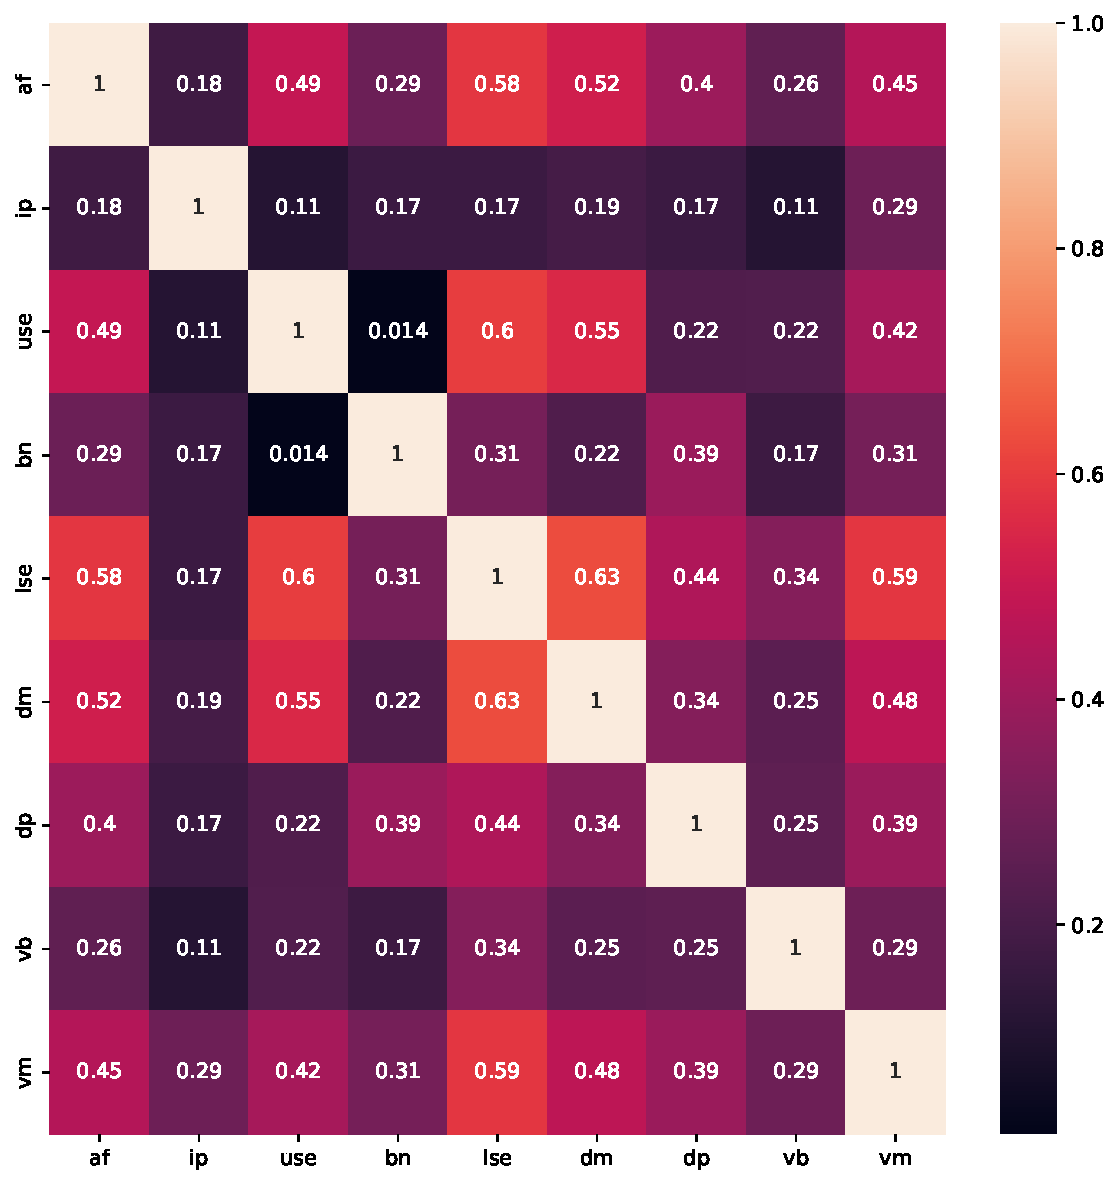
\includegraphics[width=0.6\linewidth]{../../scripts/eda/assoc_plot_tschuprow.pdf}
        \caption{Mapa de calor de la T de Tschuprow}
        \label{fig4:todd_chars__tschuprow}
    \end{subfigure}
    \caption[Mapas de calor de asociaciones entre características de Todd]{Mapas de calor que muestran las asociaciones entre las características de Todd utilizando la V de Cramér (a) y la T de Tschuprow (b). Los colores más claros indican asociaciones más fuertes entre pares de características. Los valores oscilan entre 0, lo que indica ausencia de asociación, y 1, que sugiere una asociación muy fuerte.}
    \label{fig4:todd_chars_correlogram}
\end{figure}

Si bien los datos empleados en este estudio no son de naturaleza tabular y se utilizan técnicas de DL que no requieren una extracción manual de características, resulta igualmente útil, de cara a los experimentos, analizar las asociaciones existentes entre las nueve características del método de Todd. Dado que dichas variables son categóricas, se ha optado por emplear la V de Cramér \cite{sheskin_handbook_2020}, una medida estadística que cuantifica la intensidad de la asociación entre dos variables categóricas. Un valor cercano a 1 indica una asociación fuerte entre ambas características, mientras que un valor próximo a 0 sugiere poca o ninguna asociación. Cabe destacar que la V de Cramér únicamente indica la presencia e intensidad de una relación entre variables, sin ofrecer información sobre la dirección de dicha asociación (a diferencia de las medidas de correlación para variables numéricas) \cite{jimenez_nota_2024}.

No obstante, la V de Cramér puede verse afectada por un sesgo cuando se aplica a tablas de contingencia no cuadradas, es decir, cuando el número de categorías en las variables comparadas es diferente, lo cual sucede en varias combinaciones de las características de Todd. Para corregir este efecto y obtener una interpretación más equilibrada del grado de asociación, se ha complementado el análisis con la T de Tschuprow, una medida alternativa que atenúa este sesgo y permite una comparación más justa entre pares de variables con distinta cardinalidad.

Se han generado mapas de calor por cada par de características, que pueden observarse en la Figura \ref{fig4:todd_chars_correlogram}, donde se aprecia que las asocaciones entre las características varían significativamente entre sí. Como era de esperarse, existen discrepancias ligeras entre los valores obtenidos mediante la V de Cramér y la T de Tschuprow. Para facilitar la interpretación de estos resultados, se ha incluido la Tabla \ref{table4:corr}, en la que se listan las tres características con mayor asocación para cada una.

Del análisis se concluye que las características LSE, AF y VM son, en general, las que presentan los mayores niveles de asocación con el resto, lo que sugiere una mayor dependencia entre ellas. En contraste, la característica IP muestra los niveles más bajos de asocación con las demás, seguida de BN, lo cual puede indicar un comportamiento más independiente. Este conocimiento será especialmente relevante en los experimentos de entrenamiento en modo multietiqueta, ya que incorporar características correlacionadas entre sí podría favorecer el aprendizaje del modelo y mejorar su rendimiento.

\begin{table}[t]
    \centering
    \begin{tabular}{|c|cc|}
        \hline
        \rowcolor[HTML]{D33333} 
        \cellcolor[HTML]{D33333}{\color[HTML]{FFFFFF} } & \multicolumn{2}{c|}{\cellcolor[HTML]{D33333}{\color[HTML]{FFFFFF} Características con mayor asociación}} \\ \cline{2-3} 
        \rowcolor[HTML]{D33333} 
        \multirow{-2}{*}{\cellcolor[HTML]{D33333}{\color[HTML]{FFFFFF} Característica}} & \multicolumn{1}{c|}{\cellcolor[HTML]{D33333}{\color[HTML]{FFFFFF} V de Cramér}} & {\color[HTML]{FFFFFF} T de Tschuprow} \\ \hline
        AF & \multicolumn{2}{c|}{DM, LSE, USE} \\ \cline{2-3} 
        BN & \multicolumn{1}{c|}{AF, DP, VM} & DP, LSE, VM \\ \cline{2-3} 
        DM & \multicolumn{2}{c|}{AF, LSE, USE} \\ \cline{2-3} 
        DP & \multicolumn{1}{c|}{AF, LSE, VM} & AF, BN, LSE \\
        IP & \multicolumn{1}{c|}{AF, LSE, VM} & AF, DM, VM \\
        LSE & \multicolumn{1}{c|}{AF, DM, VM} & DM, USE, VM \\ \cline{2-3} 
        USE & \multicolumn{2}{c|}{AF, DM, LSE} \\ \cline{2-3} 
        VB & \multicolumn{2}{c|}{AF, LSE, VM} \\ \cline{2-3} 
        VM & \multicolumn{1}{c|}{DM, LSE, USE} & AF, DM, LSE \\ \hline
    \end{tabular}
    \caption[Cuadro resumen de las asociaciones más fuertes entre características de Todd]{Resumen de las asociaciones más fuertes entre cada característica del método de Todd, calculadas mediante la V de Cramér y la T de Tschuprow. Para cada característica, se presentan las tres características con mayor grado de asociación. Se observa que, en algunos casos, ambos coeficientes identifican las mismas características asociadas, mientras que en otros difieren, lo que resalta la sensibilidad de cada medida frente a la estructura de las variables categóricas.}
    \label{table4:corr}
\end{table}

\subsubsection{Preparación de los datos}
\label{section4:data_preparation}
De la muestra original de 497 individuos, es decir, un total de 986 huesos correspondientes a las sínfisis del pubis izquierda y derecha, fue necesario eliminar 16 muestras por diversos motivos: presencia de deformidades anatómicas, ausencia del archivo OBJ asociado o falta de correspondencia entre el modelo 3D y los datos etiquetados provistos. Se opta por utilizar las 970 muestras restantes en su totalidad, ya que en problemas de DL es fundamental contar con un volumen de datos considerable, aunque estos estén altamente desbalanceados, pues se pueden utilizar diversas técnicas para mitigar el efecto que produce esto al rendimiento de un modelo. 

Cabe destacar que, en el caso de la característica DP (Subfigura \ref{fig4:todd_chars__dp}), el atributo 3 (\say{Presente}) cuenta con solo una muestra, lo cual impide que el modelo pueda aprender representaciones significativas para dicho atributo. Por tanto, esta muestra será eliminada durante el entrenamiento de modelos de DL que hagan uso de dicha característica. Además, el atributo 2 originalmente denominado \say{En Formación} será renombrado a \say{Presente}, con el objetivo de mantener la consistencia semántica.

Las 970 mallas presentan una resolución media de 994,601 triángulos, con un mínimo de 329,438 y un máximo de 1,688,348 triángulos. Para poder aplicar el método ExMeshCNN, descrito en la Sección \ref{section4:methods}, es necesario que todas las mallas tengan una resolución uniforme. Una opción inicial considerada fue remuestrear las mallas al número medio de triángulos; sin embargo, este tamaño resulta inviable computacionalmente con el hardware disponible.

Por esta razón, se ha procedido a reducir la resolución de las mallas a 100,000, 50,000 y 25,000 triángulos, empleando las técnicas detalladas en la Sección \ref{section4:data_reduction}. Tal como se demuestra en los experimentos descritos en la Sección \ref{section5:experiment_edge_collapse}, esta reducción no compromete significativamente la fidelidad de la superficie original. La variación entre las superficies del modelo original y las versiones reducidas es mínima, lo que permite afirmar que las mallas simplificadas conservan en mayor o menor grado parte de la información morfológica relevante para los experimentos.

Adicionalmente, el método requiere que las mallas no contengan geometría degenerada y que estén completamente selladas (es decir, que no exista geometría \textit{non-manifold} y que sea \textit{watertight}, según la terminología en gráficos por ordenador). Dado que estas mallas provienen de escaneos de objetos anatómicos reales, es esperable que algunas presenten incompletitud o defectos estructurales, lo que impide su uso directo con ExMeshCNN. Para solventar estos problemas, se aplicaron técnicas de reparación y sellado descritas en la Sección \ref{section4:data_repair}, con el objetivo de restaurar la geometría y garantizar la integridad topológica de cada modelo antes de ser procesado por la red neuronal.

\section{Métodos}
\label{section4:methods}
Como se ha mencionado previamente en la Sección \ref{section3:meshes}, ExMeshCNN \cite{kim_exmeshcnn_2022} representa el estado del arte en el procesamiento de mallas poligonales mediante DL y por lo tanto ha sido el método elegido para realizar los experimentos. A continuación se describe de qué forma el \textit{framework} adapta los datos para poder ser utilizados con convoluciones.

\subsection{Capa de descriptores}
Las representaciones en cuadrícula, como en el caso de imágenes, resultan convenientes porque encapsulan tanto la información de conectividad (es decir, la vecindad local entre píxeles) como las características asociadas (como los valores RGB) en una única estructura matricial. Sin embargo, esta estrategia no puede trasladarse directamente a las mallas tridimensionales debido a su naturaleza irregular y a la ausencia de un orden canónico entre sus elementos.

Para abordar esta limitación, se introducen dos capas iniciales en la red, denominadas descriptores, las cuales contienen parámetros entrenables. El propósito de estas capas es extraer características directamente desde la malla, independientemente del orden de sus triángulos. Estos descriptores transforman la información de la malla a un formato compatible con operaciones de convolución 1D, permitiendo que el modelo aprenda efectivamente a partir de la estructura tridimensional sin requerir una representación regular.

\subsubsection{Descriptor geodésico basado en aristas}
El objetivo de este descriptor es capturar características geodésicas locales asociadas a los triángulos de la malla, características que han sido mayoritariamente ignoradas en la literatura actual. 

Se parte del concepto de distancia geodésica entre caras, definida como el camino más corto a través de aristas que conecta el centro de un triángulo objetivo con un vértice de un triángulo adyacente, pasando por uno de los vértices del triángulo objetivo. No obstante, en mallas triangulares esta métrica resulta limitada, ya que la cantidad de aristas involucradas en dichos caminos es siempre dos, lo cual no aporta mucha información.

Para enriquecer esta representación, se incorporan ideas provenientes de la convolución geodésica propuesta por Schult et al. \cite{schult_dualconvmesh-net_2020}, que toma en cuenta no solo la longitud del camino, sino también su curvatura. De este modo, dos caminos con la misma longitud, pero distinta curvatura permiten ser diferenciados.

Sin embargo, dicha convolución geodésica presenta una limitación importante: la ambigüedad en el orden de los caminos posibles. Dado que estos no poseen una estructura de vecindad ordenada, una misma operación de convolución puede producir diferentes resultados dependiendo del orden de los elementos procesados, comprometiendo así la consistencia del aprendizaje.

Partiendo de estas ideas, se propone el siguiente descriptor $\mathcal{K}$, definido en la Ecuación \ref{eq4:geodesic}:
\begin{equation}
\label{eq4:geodesic}
    \mathcal{K}
(\bar{\textbf{a}_{t}}) = \theta_{0} \sum_{j}^{3} \textbf{u}_{t}^{j} + \theta_{1} \sum_{j}^{3}  \overrightarrow{\textbf{n}}_{t}^{j} + \theta_{2} \sum_{j}^{3} |\textbf{e}_{n(t)}^{j,1} - \textbf{e}_{n(t)}^{j,2}|
\end{equation}
Donde: 
\begin{itemize}
    \item $\bar{\textbf{a}_{t}}$ representa el conjunto conformado por un triángulo objetivo $f_{t}$ y sus tres triángulos vecinos topológicos $f_{n(t)_j}$, con $j \in \left\{1,2,3\right\}$.
    \item $\textbf{u}_{t}^{j}$ describe el vector entre el centro del triángulo $\textbf{c}_t$ y el vértice $j$-ésimo $\textbf{v}_{t}^j$ definido como  $\textbf{u}_{t}^{j} = \textbf{c}_t - \textbf{v}_t^j$ con $j \in \left\{1,2,3\right\}$.
    \item $\overrightarrow{\textbf{n}}_{t}^{j}$ es la normal del vértice $\textbf{v}_t^j$, calculada como la media de las normales de los triángulos que rodean dicho vértice.
    \item $\textbf{e}_{n(t)}^{j,k}$ representa la arista entre el vértice $\textbf{v}_{t}^j$ del triángulo objetivo y un vértice $\textbf{v}_{n(t)}^{j,k}$ del triángulo vecino, donde $k \in \left\{1,2\right\}$. Dado que solo existen dos caminos posibles desde un vértice $\textbf{v}_t^j$ hacia vértices de triángulos vecinos a través de una arista común, la diferencia $|\textbf{e}_{n(t)}^{j,1} - \textbf{e}_{n(t)}^{j,2}|$ captura una característica invariante al orden debido al valor absoluto.
    \item Los términos $\theta_0, \theta_1 $ y $\theta_2$ son parámetros entrenables por la red.
\end{itemize}


\begin{figure}
    \centering
    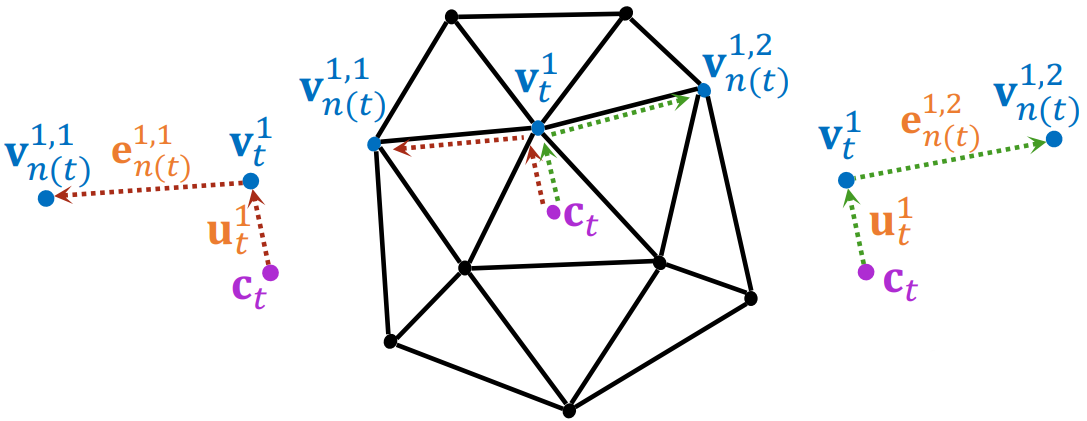
\includegraphics[width=\linewidth]{figures/4_materials-methods/geodesic_descriptor.png}
    \caption[Ejemplo visual del descriptor geodésico]{Ejemplo visual del descriptor geodésico, donde se toma como triángulo objetivo $f_t$ el que se encuentra en el centro de la malla. Se observa el vector $\textbf{u}_{t}^{1}$ que conecta el centro del triángulo $\textbf{c}_t$ con uno de sus vértices, $\textbf{v}_t^1$, así como las aristas $\textbf{e}_{n(t)}^{1,1}$ (izquierda) y $\textbf{e}_{n(t)}^{1,2}$ (derecha), que enlazan el triángulo $f_t$ con sus triángulos vecinos a través del vértice $\textbf{v}_t^1$. Este proceso se repite de forma análoga para los otros dos vértices del triángulo objetivo.}
    \label{geod_descrp}
\end{figure}

Para una mejor comprensión de estos términos, se recomienda consultar la Figura \ref{geod_descrp}. En esencia, lo que se realiza es un mapeo del triángulo objetivo y su vecindario topológico a un espacio de características geodésicas capturando las siguientes propiedades:
\begin{itemize}
    \item Forma local del triángulo, mediante el término $\textbf{u}_{t}^{j}$, que describe cómo se distribuyen espacialmente los vértices con respecto al centroide.
    \item Orientación local, reflejada en $\overrightarrow{\textbf{n}}_{t}^{j}$, que aporta información sobre la dirección normal de la superficie.
    \item Relaciones geodésicas entre triángulos vecinos, a través del término $|\textbf{e}_{n(t)}^{j,1} - \textbf{e}_{n(t)}^{j,2}|$, que captura la variación entre las conexiones posible
\end{itemize}

Además, el descriptor actúa funcionalmente como un filtro de convolución 1D de tamaño 3, ya que posee parámetros entrenables. Esto permite realizar subsiguientes convoluciones 1D sobre el vector de características obtenido.

\FloatBarrier

\subsubsection{Descriptor geométrico basado en caras}
En la literatura, las características geométricas más comúnmente empleadas para describir las caras triangulares incluyen el vector normal de la misma, su centroide y el ángulo que forma con las caras vecinas. Dado que estas características son de bajo nivel y, en cierta medida, de naturaleza heurística, se propone el descriptor $\mathcal{G}$, definido en la Ecuación \ref{eq4:geometric}, con el objetivo de capturar representaciones de alto nivel que integren dicha información geométrica.

\begin{equation}
\label{eq4:geometric}
    \mathcal{G}(\bar{\textbf{a}_{t}}) = \phi_{0} \textbf{c}_{t} + \phi_{1} \overrightarrow{\textbf{n}}_{t} + \phi_{2} \sum_{j}^{3} | \textbf{c}_{t} - \textbf{c}_{n(t)}^{j} | + \phi_{3} | \overrightarrow{\textbf{n}}_{t} \times \overrightarrow{\textbf{n}}_{n(t)}^j |
\end{equation}
Donde:
\begin{itemize}
    \item Los términos $\textbf{c}_{t}$ y $\overrightarrow{\textbf{n}}_{t}$ capturan la información relativa a la posición y orientación de la cara triangular $f_t$ en el espacio.
    \item Los términos $| \textbf{c}_{t} - \textbf{c}_{n(t)}^{j} |$ y $| \overrightarrow{\textbf{n}}_{t} \times \overrightarrow{\textbf{n}}_{n(t)}^j |$ capturan la relación que tiene el triángulo objetivo con su vecindario local respecto a la distancia entre sí y el ángulo que forman.
    \item Los términos $\phi_{0}, \phi_{1}, \phi_{2} $ y $\phi_{3}$ son parámetros entrenables por la red.
\end{itemize}

De esta forma, se logra realizar otro mapeo de las caras triangulares junto a su vecindario topológico a un espacio de características geométricas y, al igual que sucede con el descriptor de aristas, se tiene esencialmente una capa entrenable por la red y que su resultado es factible realizarle convoluciones 1D. La Figura \ref{geom_descrp} permite visualizar estos conceptos de forma clara.

\begin{figure}[hb]
    \centering
    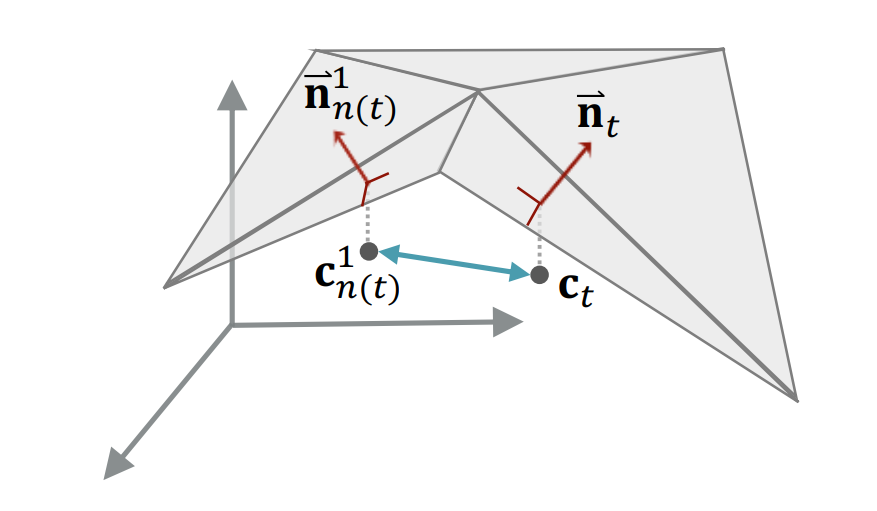
\includegraphics[width=0.75\linewidth]{figures/4_materials-methods/geometric_decriptor.png}
    \caption[Ejemplo visual del descriptor geométrico]{Ejemplo visual del descriptor geométrico, donde se muestra el triángulo objetivo $f_t$ (a la derecha de la malla) junto con su vecino topológico $f_{n(t)_1}$. Se destacan los centroides de ambos triángulos, $\textbf{c}_{t}$ y $ \textbf{c}_{n(t)}^{1}$, utilizados para calcular el vector $\left| \textbf{c}_{t} - \textbf{c}_{n(t)}^{1} \right|$, representado en azul en la figura. También se visualizan sus normales respectivas, $\overrightarrow{\textbf{n}}_{t}$ y $\overrightarrow{\textbf{n}}_{n(t)}^{1}$, cuya relación angular se captura mediante su producto cruzado.}
    \label{geom_descrp}
\end{figure}


En resumen, la primera capa de cualquier red construida con ExMeshCNN se compone de los dos descriptores $\mathcal{K}(\bar{\textbf{a}}_t)$ y $\mathcal{G}(\bar{\textbf{a}}_t)$, que funcionalmente actúan como capas convolucionales 1D pues poseen parámetros entrenables, pero que están realizando un mapeo de cada triángulo a un espacio de características geométricas y geodésicas. El resultado de los descriptores es concatenado como se observa en la Ecuación \ref{eq4:concat} para ser utilizado por las capas verdaderamente convolucionales.
\begin{equation}
    \label{eq4:concat}
    \mathcal{F}_{t} = \left[\mathcal{K}(\bar{\textbf{a}}), \mathcal{G}(\bar{\textbf{a}}) \right]
\end{equation}
Donde $\mathcal{F}_{t}$ es el vector de características de cada cara triangular. Para que estos descriptores funcionen correctamente, es necesario que las mallas estén exentas de geometría \textit{non-manifold} y sean \textit{watertight}: esto garantiza que una cara triangular siempre tendrá 3 vecinos a su alrededor, un requisito necesario para poder realizar el mapeo entre las caras triangulares y las características extraídas por los descriptores. 

\subsection{Capas convolucionales}
Dado que las mallas no poseen un orden canónico en sus triángulos, es necesario realizar un preprocesamiento antes de aplicar una operación de convolución 1D. Para ello, se expande el vector de características de cada triángulo $f_i$ de la siguiente manera:
\begin{align}
    \alpha_i &= \mathcal{F_i} \\
    \beta_i &= \sum_{j}^{3} | \mathcal{F}_{i} - \mathcal{F}_{n(i)}^{j}| 
\end{align}
Donde:
\begin{itemize}
    \item $\alpha_i$ representa las características propias del triángulo $f_i$.
    \item $\beta_i$ representa un agregado de las diferencias absolutas entre las características de $f_i$ y las de sus tres triángulos vecinos topológicos $f_{n(i)}^{j}$, con $j \in {1, 2, 3}$.
\end{itemize}

Este paso expande temporalmente el conjunto de datos, duplicando la cantidad de triángulos al generar dos entradas por triángulo: $\alpha_i$ y $\beta_i$.

Posteriormente, se aplica una convolución 1D con un kernel de tamaño 2 y un \textit{stride} de 2. Esta configuración permite que cada operación de convolución combine la información de $\alpha_i$ y $\beta_i$, de manera que la operación es invariante al orden de los triángulos en la malla. Al mismo tiempo, el uso de \textit{stride} 2 permite recuperar la dimensionalidad original del conjunto de datos.

A diferencia de otros enfoques, ExMeshCNN mantiene fijo el tamaño del filtro de convolución entre capas y controla la capacidad de la red a través de la densidad (profundidad) de las mismas. Esta arquitectura facilita el uso de técnicas de interpretabilidad como Grad-CAM, permitiendo identificar los triángulos que más contribuyen al resultado final del modelo. Adicionalmente, esta es la razón por la cual se requiere un número idéntico de caras triangulares en las mallas 3D: no se puede variar el tamaño de una capa convolucional, por lo que tiene que fijarse a un valor ya conocido de antemano.